\chapter{Zaimplementowane rozwiązanie}

Schemat przedstawiający zaprojektowany system 
przedstawiono na rysunku \ref{impl::top}:

\begin{figure}[H]
    \centering
    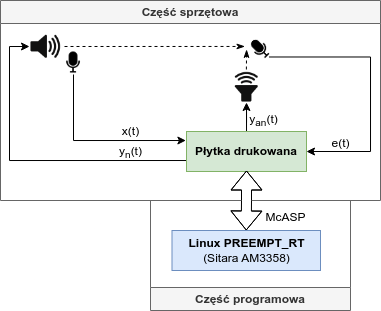
\includegraphics[width=0.75\textwidth]{graf/impl/top.png}
    \caption{Architektura systemu - najwyższy poziom}
    \label{impl::top}
\end{figure}

Na architekturę systemu składają się dwie główne części:
\begin{enumerate}

    \item Część sprzętowa - w jej skład wchodzą głośniki, mikrofony 
    oraz zaprojektowana płytka drukowana, komunikująca się z platformą
    obliczeniową.

    \item Część programowa - składa się zestawu programów działających
    w środowisku systemu operacyjnego GNU/Linux zmodyfikowanego łatką
    PREEMPT\_RT. 

\end{enumerate}
